%!TeX root=../tese.tex
%("dica" para o editor de texto: este arquivo é parte de um documento maior)
% para saber mais: https://tex.stackexchange.com/q/78101/183146

%% ------------------------------------------------------------------------- %%
\chapter{Interpretação geométrica de buscas em ABBs}
\label{cap:geometria}

Neste capítulo explicaremos a visão geométrica proposta no artigo \cite{geometry_of_bst}, o que são conjuntos de pontos arboreamente independente e como interpretar de maneira geométrica algoritmos de busca em ABBs.

\section{Conjuntos arboreamente satisfeitos}

Chamamos dois pontos $a$ e $b$ de \textit{ortogonalmente colineares} se $a$ e $b$ estão na mesma linha horizontal ou vertical. Se $a$ e $b$ não são ortogonalmente colineares, denotamos por \textit{$\{a,b\}$-retângulo} o retângulo ortogonal que tem $a$ e $b$ como vértices.

Um par de pontos $\{a,b\}$ de um conjunto de pontos $P$ é \textit{arboreamente satisfeito} se $a$ e $b$ são ortogonalmente colineares ou se há pelo menos um ponto do conjunto \( P \setminus \{a,b\} \) que está dentro da região delimitada pelo \{a,b\}-retângulo, incluindo seu perímetro. Um conjunto $P$ de pontos é \textit{arboreamente satisfeito} se todos os pares de pontos do conjunto são arboreamente satisfeitos. Veja a Figura~\ref{fig:geometria-inicial}.

\begin{figure}[h!]
    \centering
    \begin{minipage}[b]{0.45\textwidth}
        \centering
        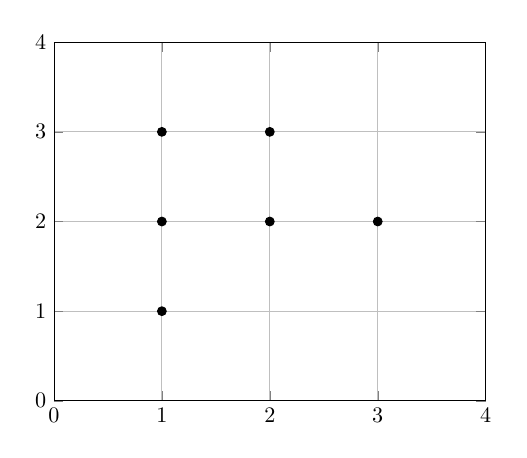
\begin{tikzpicture}[scale=0.8]
        \begin{axis}[
            grid=major,
            xmin=0, xmax=4,
            ymin=0, ymax=4,
            xtick={0,1,2,3,4},
            ytick={0,1,2,3,4}
        ]
        \addplot[only marks, mark=*] coordinates {
            (1,1)
            (1,2)
            (1,3)
            (2,2)
            (2,3)
            (3,2)
        };
        \end{axis}
        \end{tikzpicture}
    \end{minipage}\hfill
    \begin{minipage}[b]{0.45\textwidth}
        \centering
        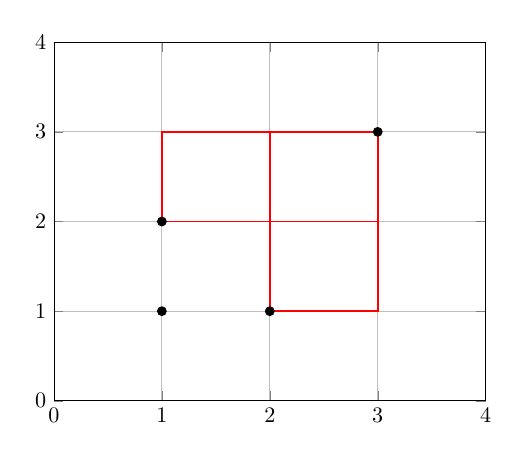
\begin{tikzpicture}[scale=0.8]
        \begin{axis}[
            grid=major,
            xmin=0, xmax=4,
            ymin=0, ymax=4,
            xtick={0,1,2,3,4},
            ytick={0,1,2,3,4}
        ]
        \addplot[only marks, mark=*] coordinates {
            (1,1)
            (1,2)
            (2,1)
            (3,3)
        };
        \addplot[
            color=red,
            line width=0.7pt
        ]
        coordinates {
            (2,1)
            (3,1)
            (3,3)
            (2,3)
            (2,1)
        };
        \addplot[
            color=red,
            line width=0.7pt
        ]
        coordinates {
            (1,2)
            (3,2)
            (3,3)
            (1,3)
            (1,2)
        };
        \end{axis}
        \end{tikzpicture}
    \end{minipage}
    \caption{À esquerda, um conjunto $P$ de pontos arboreamente satisfeito. À direita, um conjunto $P$ de pontos com dois pares de pontos arboreamente insatisfeitos com seus retângulos destacados.}
\label{fig:geometria-inicial}
\end{figure}

\begin{lemma}
\label{lem:pontos_em_arestas_incidentes}
Em um conjunto arboreamente satisfeito $P$, para todo par de pontos $\{a,b\}$ não ortogonalmente colineares, há sempre pelo menos um ponto de \( P \setminus \{a,b\} \) que está em um dos lados do $\{a,b\}$-retângulo que incide em $a$, e há sempre também pelo menos um ponto de \( P \setminus \{a,b\} \) que está em um dos lados do $\{a,b\}$-retângulo que incide em $b$.
\end{lemma}


\begin{figure}
    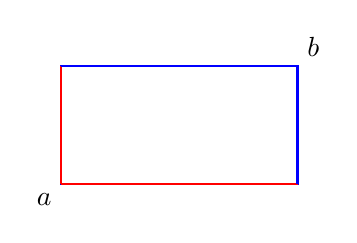
\begin{tikzpicture}[scale=1.5]
        \draw[blue, thick] (0,0) rectangle (2,1);
        
        \node at (0,0) [below left] {$a$};
        \node at (2,1) [above right] {$b$};
        
        \draw[red, thick] (0,0) -- (0,1);
        \draw[red, thick] (0,0) -- (2,0);
        \draw[blue, thick] (2,1) -- (0,1);
        \draw[blue, thick] (2,1) -- (2,0);
    \end{tikzpicture}
    \caption{O $\{a,b\}$-retângulo. Em vermelho estão destacados os lados do retângulo que incidem em $a$ e em azul estão destacados os lados que incidem em $b$.}
\end{figure}

\begin{proof} Sejam $a$ e $b$ dois pontos não ortogonalmente colineares de um conjunto arboreamente satisfeito $P$. Como $\{a,b\}$ é um par de pontos arboreamente satisfeito não ortogonalmente colineares, então a região delimitada pelo $\{a,b\}$-retângulo possui pelo menos um ponto de $P$ diferente de $\{a,b\}$. Denotemos por $c$ tal ponto. Se $c$ não estiver em um lado do $\{a,b\}$-retângulo que incide em $a$, então $a$ e $c$ não são ortogonalmente colineares e o $\{a,c\}$-retângulo está contido no $\{a,b\}$-retângulo, logo é também arboreamente satisfeito e é possível recursivamente procurar tal ponto no $\{a,c\}$-retângulo. Analogamente, se $c$ não estiver em um lado do $\{a,b\}$-retângulo que incide em $b$, então é possível recursivamente procurar tal ponto no $\{b,c\}$-retângulo, que também é arboreamente satisfeito.
\end{proof}

%Seja $\tau_i$ a subárvore // falar de subarvores?

\section{Visão geométrica de buscas}

No modelo de computação adotado, para realizar um acesso em uma ABB, o algoritmo de busca inicia o nó corrente na raiz da ABB. Em seguida, percorre a árvore descendo para o filho apropriado por meio de comparações até alcançar a chave procurada.

Dada uma sequência $X = (x_{1},\ldots,x_{m})$ de $m$ acessos às chaves $1,2,\ldots,n$, é possível ilustrar essa sequência $X$ de maneira gráfica em um plano cartesiano da seguinte forma: o eixo $x$ representará as chaves armazenadas na ABB e o eixo $y$ representará os índices $i = 1,2,\ldots,m$, que interpretamos como o tempo. Assim, um ponto de coordenada ($x$,$i$) representa a busca da chave $x$ na ABB no instante de tempo $i$, ou seja, representa $x_i$. Veja o exemplo da Figura~\ref{fig:busca_padrao}.

\begin{figure}
    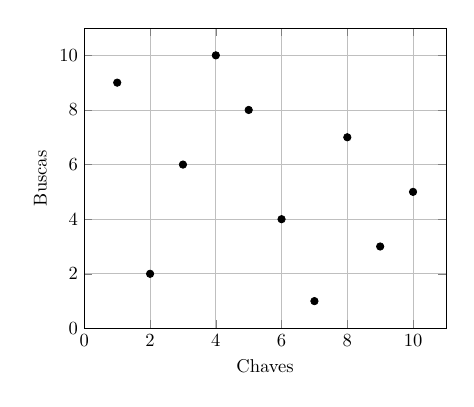
\begin{tikzpicture}[scale=0.67]
        \begin{axis}[
            xlabel={Chaves},
            ylabel={Buscas},
            grid=major,
            xmin=0, xmax=11,
            ymin=0, ymax=11,
            xtick={0,2,4,6,8,10},
            ytick={0,2,4,6,8,10}
        ]
        \addplot[only marks, mark=*] coordinates {
            (1,9)
            (2,2)
            (3,6)
            (4,10)
            (5,8)
            (6,4)
            (7,1)
            (8,7)
            (9,3)
            (10,5)
        };
        \end{axis}
    \end{tikzpicture}
    \caption{Gráfico representando a sequência (7, 2, 9, 6, 10, 3, 8, 5, 1, 4) de acessos.}
\label{fig:busca_padrao}
\end{figure}

A \textit{visão geométrica da execução de um algoritmo de busca em ABB} para uma sequência $X = (x_{1},\ldots,x_{m})$ de buscas, de maneira similar, é o conjunto de pontos na forma ($x$,$i$) tal que $x$ foi uma das chaves visitadas durante a busca pela chave $x_i$. Para cada $i \in \{1,\ldots,m\}$, o conjunto de pontos de $P$ pertencentes a reta $y = i$ representa os nós visitados durante a busca por $x_i$. Veja a Figura~\ref{fig:traducao-busca-em-ASS}.

\begin{figure}[h!]
    \centering
    \begin{minipage}[b]{0.34\textwidth}
        \centering
        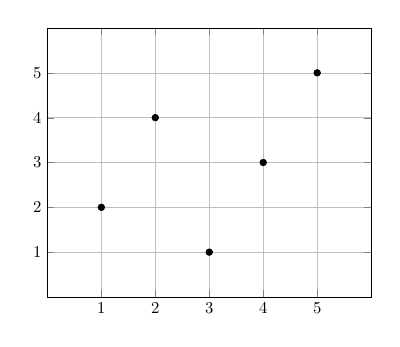
\begin{tikzpicture}[scale=0.6]
        \begin{axis}[
            grid=major,
            xmin=0, xmax=6,
            ymin=0, ymax=6,
            xtick={1,2,3,4,5},
            ytick={1,2,3,4,5}
        ]
        \addplot[only marks, mark=*] coordinates {
            (3,1)
            (1,2)
            (4,3)
            (2,4)
            (5,5)
        };
        \end{axis}
        \end{tikzpicture}
    \end{minipage}\hfill
    \begin{minipage}[b]{0.33\textwidth}
        \centering
        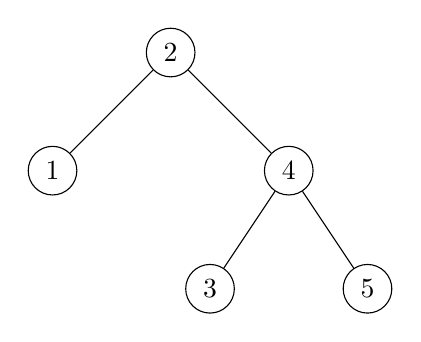
\begin{tikzpicture}
            [node/.style={circle,draw,minimum size=1.5em}]
            \node[node] (A) at (-1.5,-1.5) {$1$};
            \node[node] (B) at (0,0) {$2$};
            \node[node] (C) at (0.5,-3) {$3$};
            \node[node] (D) at (1.5,-1.5) {$4$};
            \node[node] (E) at (2.5,-3) {$5$};
            
            \draw (A) -- (B);
            \draw (B) -- (D);
            \draw (C) -- (D);
            \draw (E) -- (D);
          \end{tikzpicture}
    \end{minipage}\hfill
    \begin{minipage}[b]{0.33\textwidth}
        \centering
        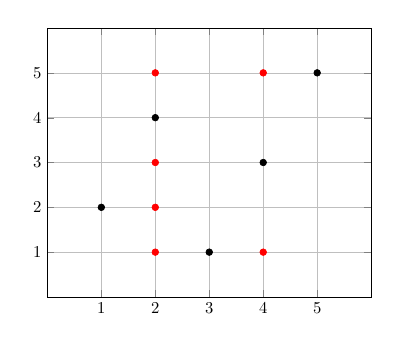
\begin{tikzpicture}[scale=0.6]
            \begin{axis}[
                grid=major,
                xmin=0, xmax=6,
                ymin=0, ymax=6,
                xtick={1,2,3,4,5},
                ytick={1,2,3,4,5}
            ]
            \addplot[only marks, mark=*] coordinates {
                (3,1)
                (1,2)
                (4,3)
                (2,4)
                (5,5)
            };
            \addplot[color=red, only marks, mark=*] coordinates {
                (2,1)
                (4,1)
                (2,2)
                (2,3)
                (2,5)
                (4,5)
            };
            \end{axis}
            \end{tikzpicture}
    \end{minipage}
    \caption{À esquerda, o conjunto de pontos que representa a sequência $X = (3,1,4,2,5)$. No meio, uma possível ABB com as chaves \{1,2,\ldots,5\}. À direita, o conjunto correspondente aos nós da ABB ao centro, visitados pelo algoritmo de busca que não efetua rotações. Os pontos pretos são os nós da sequência $X$ de acessos e os pontos vermelhos são o restante dos nós visitados durante cada um desses acessos. Note que o conjunto de pontos à esquerda não é arboreamente satisfeito, mas o conjunto à direita é.}
\label{fig:traducao-busca-em-ASS}
\end{figure}

\begin{lemma} A visão geométrica de qualquer execução de um algoritmo de busca em ABB no modelo de computação adotado é um conjunto de pontos arboreamente satisfeitos.
\label{lema:visao_geometrica_vira_ASS}
\end{lemma}

\begin{proof}
Suponha, por contradição, que a visão geométrica de um algoritmo de busca em uma ABB $T$ não é um conjunto arboreamente satisfeito. Dessa maneira, há pelo menos um par $\{p,q\}$ de pontos nesse conjunto que não é arboreamente satisfeito, onde $p = (a,i)$ e $q = (b,j)$. Assumiremos sem perda de generalidade que $i < j$ e $a < b$.

Os quatro lados do $\{p,q\}$-retângulo terão um papel a seguir na prova. São eles:
\begin{itemize}
    \item $\ell_1$ = \{$(x,y)$ | $x = a$ e $i < y \leq j$\},
    \item $\ell_2$ = \{$(x,y)$ | $a \leq x < b$ e $y = j$\},
    \item $\ell_3$ = \{$(x,y)$ | $x = b$ e $i \leq y < j$\},
    \item $\ell_4$ = \{$(x,y)$ | $a < x \leq b$ e $y = i$\},
\end{itemize}
onde $\ell_1$ representa as visitas à chave $a$ entre os instantes de tempo $i$ e $j$, $\ell_2$ as visitas às chaves entre $a$ e $b$ no instante de tempo $j$, $\ell_3$ as visitas à chave $b$ entre os instantes de tempo $i$ e $j$ e $\ell_4$ as visitas às chaves entre $a$ e $b$ no instante de tempo $i$.

Como $\{p,q\}$ é um par de pontos arboreamente insatisfeito, nota-se que não há nenhum ponto tanto nas bordas quanto no interior do $\{p,q\}$-retângulo. Logo, $\ell_1 \cup \ell_2 \cup \ell_3 \cup \ell_4 = \emptyset$.

Sejam $e$, $f$ e $g$ chaves dos nós $E$, $F$ e $G$ de uma ABB. Note que se o $F$ é o ancestral comum mais profundo dos nós $E$ e $G$, então sabemos que $e \leq f \leq g$ e, mais importante, $F$ é ancestral dos nós $E$ e $G$ nesta ABB, e assim os nós $E$ e $G$ têm profundidade maior que~$F$. Logo, $F$ está no caminho da raiz desta ABB até qualquer chave no intervalo $[e,g]$. Em outras palavras, para visitar qualquer nó da ABB com chave no intervalo $[e,g]$, é necessário visitar o ancestral comum mais profundo entre $E$ e $G$ que neste caso é $F$.

No que segue, abusaremos da notação e usaremos um valor $x$ em $[1,n]$ para nos referimos tanto a uma chave $x$ como ao nó de $T$ que armazena $x$.

Seja $c$ o ancestral comum mais profundo de $a$ e $b$ em $T$ imediatamente antes da busca $i$. Seja $d$ o ancestral comum mais profundo de $a$ e $b$ em $T$ imediatamente antes da busca $j$.

\begin{figure}[H]
    \centering
    \vfill % Adiciona espaço acima da figura para centralização vertical
    \begin{minipage}[t]{0.6\textwidth}
        Como $\ell_2 = \emptyset$, então obrigatoriamente $d = b$. Por outro lado, como $\ell_3 = \emptyset$, temos que $c \neq b$ e, em algum instante de tempo $h$, com $i \leq h < j$, $b$ teve que ser visitado para ser rotacionado e se tornar o ancestral comum mais profundo entre $a$ e $b$ no instante $j$, logo $\ell_3 \neq \emptyset$ e concluímos que $\ell_2 \cup \ell_3 \neq \emptyset$.

        Como $\ell_4 = \emptyset$, então $c = a$. Porém, no instante $j$, $b$ é acessado. Caso $c = d = a$, $a$ precisa ser visitado no instante de tempo $j$, logo $\ell_1 \neq \emptyset$. Caso $c \neq d$, então em algum instante de tempo $h$, com $i \leq h < j$, o ancestral comum mais profundo entre $a$ e $b$ mudou. Logo algum nó com chave no intervalo $(a,b]$ precisa ter sido rotacionado para se tornar o novo ancestral comum mais profundo entre $a$ e $b$. Porém sabemos que para visitar qualquer chave no intervalo $[a,b]$ no instante de tempo $h$, é necessário visitar o ancestral comum mais profundo entre $a$ e $b$, que neste caso é $a$. Logo $\ell_1 \neq \emptyset$ e concluímos que $\ell_1 \cup \ell_4 \neq \emptyset$.
    \end{minipage}\hfill
    \begin{minipage}[t]{0.4\textwidth}
        % Coluna da direita com a imagem e a legenda
        \centering
        \begin{figure}[H]
            \centering
            \begin{adjustbox}{valign=t, raise=-55pt} % Alinha o gráfico ao topo da caixa
            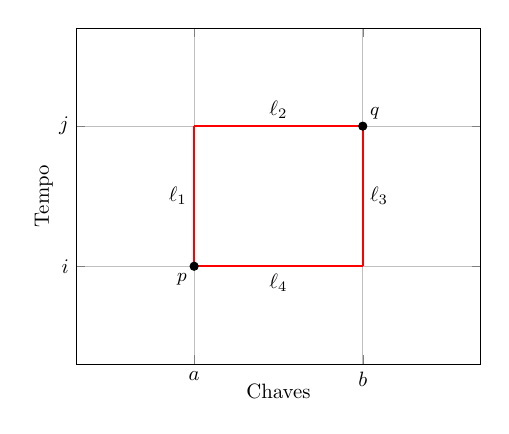
\begin{tikzpicture}[scale=0.75]
            \begin{axis}[
                xlabel={Chaves},
                ylabel={Tempo},
                grid=major,
                xmin=0.3, xmax=2.7,
                ymin=0.3, ymax=2.7,
                xtick={1,2},
                ytick={1,2},
                xlabel style={at={(axis description cs:0.5,-0.08)}, anchor=center}, % Ajusta a posição do rótulo do eixo x
                ylabel style={at={(axis description cs:-0.08,0.5)}, anchor=center},
                xticklabels={$a$,$b$}, % Define os rótulos do eixo x
                yticklabels={$i$,$j$} % Define os rótulos do eixo y
            ]

            \addplot[only marks, mark=*] coordinates {
                (1,1)
                (2,2)
            };

            \addplot[red, thick] coordinates {
                (1,2)
                (2,2)
            };

            \addplot[red, thick] coordinates {
                (2,2)
                (2,1)
            };

            \addplot[red, thick] coordinates {
                (1,1)
                (1,2)
            };

            \addplot[red, thick] coordinates {
                (1,1)
                (2,1)
            };

            % Adiciona rótulos aos pontos
            \node at (axis cs:1,1) [anchor=north east, fill=white, font=\small] {$p$};
            \node at (axis cs:2,2) [anchor=south west, fill=white, font=\small] {$q$};

            \node at (axis cs:1,1.5) [anchor=east, font=\normalsize] {$\ell_1$};
            \node at (axis cs:1.5,2) [anchor=south, font=\normalsize] {$\ell_2$};
            \node at (axis cs:2,1.5) [anchor=west, font=\normalsize] {$\ell_3$};
            \node at (axis cs:1.5,1) [anchor=north, font=\normalsize] {$\ell_4$};
            %\node at (axis cs:1.5,1.5) [anchor=center, font=\normalsize] {5};

            \end{axis}
            \end{tikzpicture}
            \end{adjustbox}
            \label{fig:tikz-captions}
        \end{figure}
    \end{minipage}
    \vfill % Adiciona espaço abaixo da figura para centralização vertical
    \label{fig:chaves-buscas}
\end{figure}

Por contra-positiva das conclusões acima, temos:
\begin{center}
Se $\ell_3 = \emptyset$, então $\ell_2 \neq \emptyset$. \\
Se $\ell_1 = \emptyset$, então $\ell_4 \neq \emptyset$.
\end{center}

Conclui-se então que $\ell_1 \cup \ell_4  \neq \emptyset$ e $\ell_2 \cup \ell_3  \neq \emptyset$, e assim chegamos numa contradição.

Vale ressaltar que, pelo Lema~\ref{lem:pontos_em_arestas_incidentes}, $\ell_1 \cup \ell_4  \neq \emptyset$ e $\ell_2 \cup \ell_3  \neq \emptyset$, uma vez que $\ell_1 \cup \ell_4$ representa os pontos pertencentes aos lados do $\{p,q\}$-retângulo incidentes ao vértice $p$ e  $\ell_2 \cup \ell_3$ representa os pontos pertencentes aos lados do $\{p,q\}$-retângulo incidentes ao vértice~$q$.
\end{proof}

A partir daqui, consideraremos apenas pontos $(x,y)$ em que $x$ e $y$ são inteiros, $1 \leq x \leq n$ e $1 \leq y \leq m$.

\begin{lemma}Qualquer conjunto de pontos arboreamente satisfeito representa a execução de um algoritmo de busca em ABB no modelo de computação adotado.
\end{lemma}

\begin{proof}
Usaremos um tipo de árvore binária de busca denominada \textit{treap}. Os nós de uma treap possuem dois campos, um chamado chave e outro chamado prioridade. A treap mantém duas propriedades: a propriedade de ordem de árvores binárias de busca em relação às chaves e a propriedade de heap em relação às prioridades. Assim, todo nó de uma treap possui chave maior que os nós da sua subárvore esquerda e chave menor que os nós da sua subárvore direita. Além disso, os nós da treap obedecem à propriedade de heap, que pode ser de dois tipos: se for um heap máximo, cada nó terá prioridade maior ou igual a de seus filhos; se for um heap mínimo, cada nó terá prioridade menor ou igual a de seus filhos.

Seja $P$ um conjunto de pontos arboreamente satisfeito. Denotaremos por $N(h,i)$ a coordenada $y$ do ponto mais baixo do conjunto que possui coordenadas $x = h$ e $y > i$. Caso não exista tal ponto, definiremos $N(h,i) = \infty$. Assim, 
\[
N(h,i) = 
\begin{cases}
    \min\{y : (h,y) \in P \text{ e } y > i\} & \text{se tal ponto existe,} \\
    \infty & \text{caso contrário.}
\end{cases}
\]

%(Denotaremos por $N(h,i)$ a coordenada $y$ do ponto $q$ com menor distância em relação ao ponto $(h,i)$ tal que $q \in P$ e $q \in r$, onde $r$ = \{$(x,y)$ | $x = h$ e $y > i$\}.) - Escrevi essa definição alternativa que é um pouco mais formal, apesar de ser menos clara. Não sei se ficou melhor.


%Vale ressaltar que por conta da propriedade de heap em relação às prioridades dos nós, se uma subárvore conexa da treap com nós de mesma prioridade existir, então é possível realocar os nós dessa subárvore de maneira arbitraria em relação à prioridade sem desobedecer a propriedade de heap seguida pela treap. Assim, se for possível encontrar uma subárvore conexa com nós de mesma prioridade em uma treap, então existem mais de uma treap válida para este conjunto de nós e, portanto, essa treap não é única.

É possível criar uma treap que é um heap mínimo nas prioridades a partir de $P$. Para cada $j$ no intervalo $[1,n]$, adicione um nó na forma ($j$, $N(j,0)$), ou seja, adicione um nó com chave $j$ e prioridade $N(j,0)$. Essa é a nossa treap inicial.

Com essa treap criada, nota-se que já temos uma ABB que possui $n$ nós. Se conseguirmos provar que, para cada instante de tempo $h$, variando de $1$ a $m$, visitamos todos os nós com chave $z$ tal que $(z,h) \in P$ e reestruturamos a treap de maneira a manter sua estrutura sem visitar nós extras, então descrevemos uma execução de um algoritmo offline de busca em uma ABB no modelo de computação adotado.

Primeiramente, note que os nós com prioridade mínima induzem uma subárvore da treap que contém a raiz.
Seja $i$ essa prioridade mínima. Os nós com prioridade $i$ serão visitados no instante $i$ e terão sua prioridade alterada apenas considerando essa subárvore. Queremos mostrar que, ao fazer tais alterações nas prioridades no instante $i$ e reorganizar a treap dessa maneira, a treap toda continua satisfazendo a propriedade de heap.

Vamos supor, por contradição, que há um nó $q$ cuja prioridade é menor que de seu pai $p$ na treap após as modificações do instante $i$. Isso só pode ocorrer se $p$ estiver dentro da subárvore dos nós visitados no instante $i$ e $q$ não estiver nessa subárvore. Seja $a$ a chave de $p$ e $b$ a chave de $q$ e assumiremos sem perda de generalidade que $a < b$. Assim, $N(a,i) > N(b,i)$. Veja a Figura~\ref{fig:representacao_grafica}.

%que há dois nós, $p$ com chave $a$ e $q$ com chave $b$ ($a \neq b$), tal que o nó $p$ está contido na subárvore dos nós visitados no instante de tempo $i$ e o nó $q$ não foi visitado no instante de tempo $i$ e sua prioridade é menor que . Assim, $N(a,i) > N(b,i)$. Assumiremos sem perda de generalidade que $a < b$ e que $p$ é pai de $q$ durante o instante de tempo $i$. Veja a Figura~\ref{fig:representacao_grafica}.

\begin{figure}[H]
    \begin{tikzpicture}
        \coordinate (A) at (0, 0);
        \coordinate (B) at (3, 0);
        \coordinate (C) at (1.5, 2.6);
    
        \draw (A) -- (B) -- (C) -- cycle;
    
        \path (A) ++(0,1) coordinate (start);
        \path (start) ++(3,0.7) coordinate (end);
        \draw[dashed] (start) -- (end) node[midway,below] {};
    
        \path (start) ++(1.5,0.57) coordinate (x);
        \path (start) ++(1.7,0.2) coordinate (y);

        \begin{scope}
            \clip (A) -- (B) -- (C) -- cycle; % Clipping para definir a área do triângulo
            \fill[pattern=vertical lines] (A) -- (C) -- (end) -- (start) -- cycle; % Preenchimento hachurado
        \end{scope}
    
        %\filldraw (x) circle (2pt) node[anchor=south] {};
        %\filldraw (y) circle (2pt) node[anchor=north] {};
    
        \draw[red, thick] (x) -- (y);

        \filldraw (x) circle (1.5pt) node[anchor=south] {$p$};
        \filldraw (y) circle (1.5pt) node[anchor=north] {$q$};

        \draw[->, black] (1.8,1.8) -- (2.5,2) node[pos=1, right] {Nós visitados no instante de tempo $i$};
    \end{tikzpicture}
    \caption{Representação da situação descrita. O triângulo é uma representação simplificada de uma ABB. A área destacada representa todos os nós acessados no instante de tempo $i$. O nó $q$ não foi visitado nesse instante de tempo.}
\label{fig:representacao_grafica}
\end{figure}

De maneira informal, os nós $p$ e $q$ são nós pai-filho. Durante o instante de tempo $i$, $p$ será visitado pelo algoritmo de busca e o nó $q$ não. Após o instante $i$, queremos visitar o nó $q$ pela primeira vez no instante $j = N(b,i)$ antes de fazer qualquer outra visita ao nó $p$, porém isso é impossível. Vamos mostrar que, neste caso, $P$ não era um conjunto arboreamente satisfeito.

Os lados a seguir terão um papel na prova e estão representados na Figura~\ref{fig:area_delimitada}. São eles:
\begin{itemize}
    \item $\ell_1$ = \{$(x,y)$ | $x = a$ e $i < y \leq j$\}, e
    \item $\ell_2$ = \{$(x,y)$ | $a < x \leq b$ e $y = i$\},
\end{itemize}
onde $\ell_1 = \emptyset$, pois o nó $p$ não é visitado entre os instantes de tempo $i+1$ e $j$, e $\ell_2$ representa todas as visitas aos nós com chave no intervalo $(a,b]$ no instante de tempo $i$.

Denotemos por $r$ o ponto com coordenadas $(a,i)$ e por $s$ o ponto com coordenadas $(b,j)$. De acordo com a suposição feita, ambos estes pontos pertencem a $P$.
\begin{figure}
    \centering
    \begin{adjustbox}{valign=t, raise=-25pt} % Alinha o gráfico ao topo da caixa
    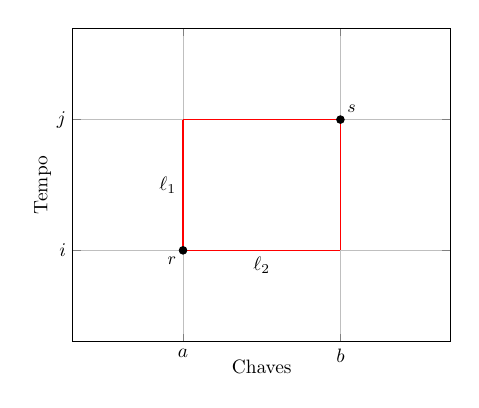
\begin{tikzpicture}[scale=0.7]
    \begin{axis}[
        xlabel={Chaves},
        ylabel={Tempo},
        grid=major,
        xmin=0.3, xmax=2.7,
        ymin=0.3, ymax=2.7,
        xtick={1,2},
        ytick={1,2},
        xlabel style={at={(axis description cs:0.5,-0.08)}, anchor=center}, % Ajusta a posição do rótulo do eixo x
        ylabel style={at={(axis description cs:-0.08,0.5)}, anchor=center},
        xticklabels={$a$,$b$}, % Define os rótulos do eixo x
        yticklabels={$i$,$j$} % Define os rótulos do eixo y
    ]

    \addplot[only marks, mark=*] coordinates {
        (1,1)
        (2,2)
    };

    \addplot[red, thick] coordinates {
        (1,2)
        (2,2)
    };

    \addplot[red, thick] coordinates {
        (2,2)
        (2,1)
    };

    \addplot[red, thick] coordinates {
        (1,1)
        (1,2)
    };

    \addplot[red, thick] coordinates {
        (1,1)
        (2,1)
    };

    % Adiciona rótulos aos pontos
    \node at (axis cs:1,1) [anchor=north east, fill=white, font=\small] {$r$};
    \node at (axis cs:2,2) [anchor=south west, fill=white, font=\small] {$s$};

    \node at (axis cs:1,1.5) [anchor=east, font=\normalsize] {$\ell_1$};
    \node at (axis cs:1.5,1) [anchor=north, font=\normalsize] {$\ell_2$};

    \end{axis}
    \end{tikzpicture}
    \end{adjustbox}
    \caption{Representação no conjunto $P$ da situação descrita.}
\label{fig:area_delimitada}
\end{figure}

Como $r,s \in P$, então $\{r,s\}$ representa um par de pontos arboreamente satisfeito. De acordo com o Lema~\ref{lem:pontos_em_arestas_incidentes}, há pelo menos um outro ponto de $P$ em alguma das arestas do $\{r,s\}$-retângulo que incide em $r$. Como o lado $\ell_1 = \emptyset$, pelo Lema~\ref{lem:pontos_em_arestas_incidentes} ser verdadeiro para $P$, $\ell_2 \neq \emptyset$, ou seja, é necessário ter um ponto de $P$ no lado $\ell_2$ e consequentemente, algum nó com chave no intervalo $(a,b]$ deve ter sido visitado durante o instante de tempo $i$.

Como $q$ é filho direito de $p$, então qualquer nó de chave no intervalo ($a,b$) no instante de tempo $i$, pela propriedade da ordenação de ABBs, está na subárvore esquerda do nó $q$. Assim,

é necessário acessar ambos os nós $p$ e $q$, pois esses nós são mais superficiais e estão no caminho entre a raiz da ABB e os nós de chave no intervalo ($a,b$).

Assim, como o par de pontos $\{r,s\}$ é arboreamente satisfeito, algum nó com chave no intervalo ($a,b$) foi visitado no instante de tempo $i$, porém para acessar um nó com chave neste intervalo no instante de tempo $i$ é preciso acessar a chave $b$, e a suposição inicial era que $b$ não era visitada neste instante de tempo. Chegamos numa contradição.

Assim, nota-se que a reestruturação da treap da maneira proposta é sempre válida em conjuntos de pontos arboreamente satisfeitos e tal reestruturação descreve um algoritmo offline que converte um conjunto de pontos arboreamente satisfeitos em uma execução de um algoritmo de busca em ABB dentro do modelo de computação adotado.
\end{proof}


% Basicamente é uma prova por indução. Precisamos provar que se era válida, se tornará válida. Assim, se tiver o problema de dois pontos estarem insatisfeitos, então a treap inicial tinha um elemento embaixo de q que deveria ter sido visitado no instante $i$, ou seja, a treap não era válida.

